\section{Arquitectura}

En la figura \ref{fig:arquitectura} se muestra el diagrama de la arquitectura propuesta con la que se trabajará para solucionar la problemática.

%En la figura \ref{fig:arquitectura} se describirá la arquitectura propuesta para la solución de la problemática.

\begin{figure}[htb]
	\centering
	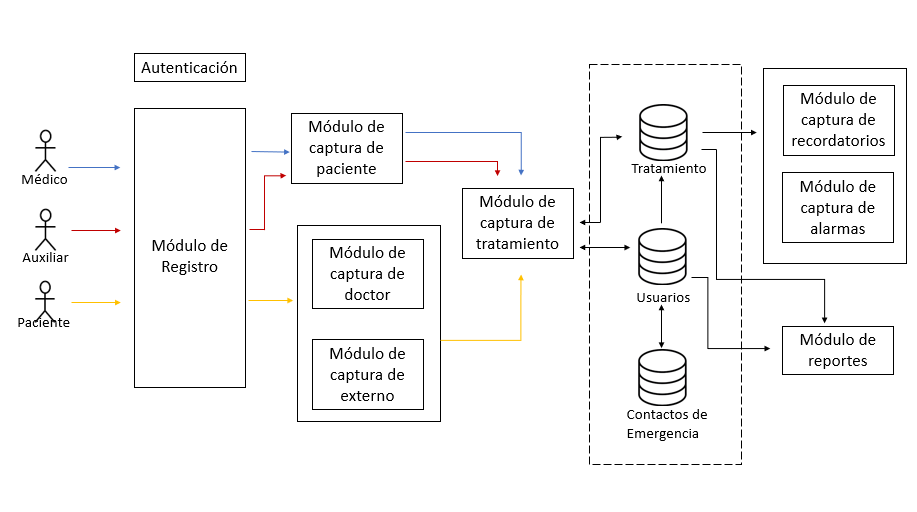
\includegraphics[width=0.8\textwidth]{images/cap2/Arquitectura}
	\caption{Arquitectura} \label{fig:arquitectura}
\end{figure}

Como podemos notar en la figura \ref{fig:arquitectura} se cuenta con cuatro roles que participarán en el sistema, los cuales son :
\begin{itemize}
	\item Administrador: Dentro del sistema, el rol \textbf{Administrador} será el encargado de ingresar los medicamentos a la base de datos, ya que estos son la base para los tratamientos del paciente.
	Las acciones con las que cuenta su rol son:
	\begin{itemize}
		\item Agregar medicamento.
		\item Eliminar medicamento.
		\item Consultar medicamento.
		\item Editar medicamento.
	\end{itemize}
	
	
	\item Paciente: Se le llama paciente a la persona que cuenta con un diagnostico generado por el \textbf{Médico} que se encuentra a cargo de su salud.\\
	
	Las acciones con las que cuenta su rol son:
	\begin{itemize}
		\item Consultar sus tratamientos médicos.
		\item Agregar el tratamiento médico.
		\item Modificar el tratamiento médico.
		\item Eliminar el tratamiento médico.
		\item Consultar sus doctores.
		\item Asociar doctor.
		\item Eliminar doctor.
		\item Consultar sus auxiliares.
		\item Asociar auxiliar.
		\item Eliminar auxiliar.
		\item Consultar sus contactos de emergencia.
		\item Asociar contacto de emergencia.
		\item Eliminar contacto de emergencia.
		\item Editar recordatorios.
		\item Consultar sus datos.
		\item Actualizar sus datos.
	\end{itemize}

	\item Médico: \\ \textbf{Médico} dentro del sistema es el profesional de la salud que se encarga del diagnostico del paciente.
	Las acciones con las que cuenta su rol son:
		\begin{itemize}
			
			\item Consultar sus pacientes.
			\item Consultar el tratamiento de sus pacientes.
			\item Modificar el tratamiento de sus pacientes.
			\item Eliminar el tratamiento médico de sus pacientes.
			\item Asociar nuevo paciente.
			\item Agregar tratamiento a un nuevo paciente.
			\item Editar notificaciones.
			\item Consultar historial clínico.
			\item Eliminar un paciente.
			\item Modificar un paciente.
			
%			\item consultar el total de pacientes que tiene.
%			\item agregar un tratamiento medico a sus pacientes.
%			\item modificar un tratamiento medico a sus pacientes.
%			\item eliminar un tratamiento medico a sus pacientes.
%			\item consultar el tratamiento medico de sus pacientes.
%			\item consultar el historial medico de sus pacientes.
%			\item agregar un paciente.
%			\item modificar un paciente.
%			\item eliminar un paciente.
		\end{itemize}

	\item Auxiliar: nace de la necesidad de ayudar a los pacientes que cuentan con poca o nula experiencia los dispositivos móviles o que por factores ajenos a la aplicación como son la edad o alguna enfermedad, les sea imposible utilizar la aplicación por si mismos\\
	Las acciones con las que cuenta su rol son:
	\begin{itemize}
		\item Consultar sus pacientes.
		\item Registrar sus tratamientos.
		\item Modificar sus tratamientos.
		\item Eliminar sus tratamientos.
		\item Editar sus notificaciones.
		\item Consultar sus doctores.
		\item Asociar doctor.
		\item Eliminar doctor.
		\item Consultar sus contactos de emergencia.
		\item Asociar contactos de emergencia.
		\item Eliminar contactos de emergencia.
%		
%		\item Agregar Paciente.
%		\item Modificar Paciente.
%		\item Eliminar Paciente.
%		\item Agregar Tratamiento medico.
%		\item Modificar Tratamiento medico.
%		\item Consultar Tratamiento medico.
%		\item Modificar notificación
	\end{itemize}
\end{itemize}


\section{Módulos}
La arquitectura contará con los siguientes módulos:
\begin{itemize}
	\item Módulo de Registro: Este módulo es el encargado de registrar e ingresar a los actores dentro de la aplicación. 
	
	
	\item Módulo de Autenticación: Una vez que te hayas registrado dentro de la aplicación, el módulo de autenticación se encargará de verificar tu perfil y habilitar los módulos correspondientes.
	
	 
	\item Módulo de captura de paciente: Este módulo es el encargado de agregar al paciente con el que trabajarán el doctor y el auxiliar.
	
	\item Módulo de captura de doctor: Este módulo es el encargado de agregar al doctor que está a cargo del tratamiento del paciente.
	
	\item Módulo de captura de auxiliar: Este módulo es el encargado de agregar al auxiliar que está a cargo del tratamiento del paciente.
	
	\item Módulo de captura de tratamiento: Este módulo es el encargado de ingresar el tratamiento médico del paciente y con el que podrán trabajar tanto el doctor como el auxiliar. 
%	y lo asociara al perfil del paciente con la información correspondiente del tratamiento.
	
	\item Módulo de recordatorios: Este módulo es el encargado de crear los recordatorios para tomar los medicamentos que se ingresaron en el tratamiento.
	
	\item Módulo de alarmas: Este módulo es el encargado de crear las alarmas cuando la situación del paciente sea delicada o que la toma de un medicamento sea de alta prioridad.
	
	\item Módulo de reportes: Este módulo es el encargado de generar un reporte con la información del tratamiento y datos relevantes del paciente como lo son la edad, estatura, peso, etc.
	
	
	
	
	
%	\item Módulo de Autenticación: El modulo encargado de verificar tu perfil y darte acceso a los módulos correspondientes.
%	\item Módulo captura de tratamientos: El modulo encargado de ingresar el tratamiento medico y lo asociara al perfil del paciente con la información correspondiente del tratamiento.
%	\item Módulo de recordatorios: Una vez que se paso por el modulo de \textbf{Captura de tratamiento} llegamos al modulo de recordatorios en donde se generaran los notificaciones a partir de la información obtenida del modulo de captura de tratamiento.
%	\item Módulo de alarmas: Este modulo es el encargado de cuando una notificación no haya sido silenciada esta se convierta en una alarma que le estará recordando al paciente tomar su medicamento.
%	\item Módulo de reportes: El modulo de reportes sirve para notificar al medico y al paciente que tan constante ha sido con su tratamiento.
%	\item Módulo de estadísticas: 
\end{itemize}


\section{Requerimientos}
Los requerimientos funcionales describen lo que el sistema debe hacer. Son declaraciones de los servicios que debe proporcionar el sistema, de la manera en que éste debe reaccionar a entradas particulares y de cómo se debe comportar en situaciones particulares.\\
En la siguiente sección se especificarán los requerimientos con los que estará trabajando la aplicación.\\
\begin{itemize}
		\item RF1 - Registro de Usuario
		La aplicación permitirá el registro de nuevos usuarios mediante el ingreso de su nombre, correo electrónico y contraseña.
		
		\item RF2 - Acceso al Sistema.
		La aplicación permitira el acceso al sistema proporcionando el correo electrónico y la contraseña con la que se registraron en la aplicación
		
		Los usuarios accederán al sistema proporcionando el correo electrónico y la contraseña con la que se registraron en la aplicación
		
		\item RF3 - Agregar Paciente.
		 
		 La aplicación permitirá que tanto el doctor como el auxiliar agreguen a los pacientes con los que están trabajando a la \textbf{lista de pacientes}.
		 
		El usuario doctor agregará a un paciente a su \textbf{lista de pacientes} ingresando el correo electrónico o nombre del paciente.
		El usuario auxiliar agregará a un paciente a su \textbf{lista de pacientes} ingresando el correo electrónico o nombre del paciente.
		El usuario paciente agregará a un doctor a su \textbf{lista de doctores} ingresando el correo electrónico o nombre del paciente.
		El usuario paciente agregará a un doctor a su \textbf{lista de auxiliares} ingresando el correo electrónico o nombre del paciente.
	
		\item RF4 - Agregar Doctor o Auxiliar.
		
		La aplicación permitirá al Paciente agregar al doctor que receto su tratamiento a su \textbf{lista de doctores} y en el caso de que sea necesario, agregar a la \textbf{lista de auxiliares} a un auxiliar para que sea el encargado de su tratamiento.
		
		\item RF5 - Alta de Invitación.
		
		Cuando un usuario haya agregado a otro usuario, la aplicación mandará un correo con el cual se vincularán sus perfiles.
		
		\item RF6 - Agregar Tratamiento.
		
		La aplicación permitirá  ya sea al doctor, auxiliar o paciente agregar el tratamiento expedido por el doctor al perfil del paciente en cuestión.
		
		\item RF7 - Creación de Recordatorios.
		
		La aplicación creará los recordatorios de los medicamentos a tomar  una vez que el tratamiento haya sido ingresado en el sistema.
		
		\item RF8 - Creación de Alarmas.
		
		La aplicación permitirá al usuario configurar alarmas cuando el ingerir un medicamento sea de suma importancia.
		
		\item RF9 - Gestión de Contactos de Emergencia.
		
		Cuando una notificación de un medicamento con un alta importancia no haya sido silenciada después de tres intentos, la aplicación mandará un mensaje a los contactos de emergencia.
		
		\item RF10 - Creación de reportes.
		
		La aplicación permitirá al usuario ingresar datos relevantes de su salud y creará un reporte con el avance de sus tratamientos los datos ingresados.
\end{itemize}


Requerimientos No Funcionales
\begin{itemize}
	\item RNF-1 Creación de Usuario
	La creación del usuario dependerá del perfil que tenga, esto quiere decir que el formulario que llenará un doctor es distinto el de un paciente.
	\item RNF-2 Verificación de Perfil
	La aplicación deberá de distinguir entre los 4 tipos de perfiles que hay, los cuales son: Paciente, Auxiliar, Doctor y Administrador.
	\item RNF-3 Gestión de Recordatorios.
	La aplicación creara los recordatorios con un mensaje que se desplegará en la pantalla y emitirá un sonido al ser enviado.
	\item RNF-4 Interfaz Comprensible.
	La aplicación contará con una interfaz entendible para un niño hasta una persona de la tercera edad y para lograr esto se trabajará con respecto a los iconos, botones y el flujo de la aplicación.
	\item RNF-5 Base de datos.
	La aplicación contará con una base de datos de forma local que permitirá que la consulta de los datos sea más rápida.
	\item RNF-6 Desarrollo Multiplataforma.
	La aplicación sera desatollada para los sistemas operativos iOs y Android siendo una aplicación nativa permitiendo asi explotar todas sus ventajas.
	\item RNF-7 Desempeño Web y Móvil.
	La aplicación permitirá que el registro del tratamiento sea ingresado por una pagina web o mediante la aplicación movil. 
	\item RNF-8	Protección de Información
	La aplicación contará con un cifrado AES-128 para proporcionar toda la seguridad a la información del usuario.
\end{itemize}





	
	\subsection{Módulo de Registro}
RF1 - Registro de Usuario
La aplicación permitirá el registro de nuevos usuarios mediante el ingreso de su nombre, correo electrónico y contraseña.
	
	\begin{ReqUser}		
		\reqUserItem{RU-MR1}{Registro de Usuario}{
			El usuario requiere de un mecanismo que le permite registrarse en la aplicación}
		{\alta}{}{\corregir}
	\end{ReqUser}

	\begin{ReqUser}		
		\reqUserItem{RU-MR2}{Acceso al Sistem}{
			El usuaio requiere de un mecanismo que le permita ingresar al sistema.}
		{\alta}{}{\corregir}
	\end{ReqUser}


	\begin{ReqUser}		
		\reqUserItem{RU-MR3}{Recuperar Contraseña}{
			El usuaio requiere de un mecanismo que le permita recuperar su contraseña o crear una contraseña nueva.}
		{\alta}{}{\corregir}
	\end{ReqUser}


	\begin{ReqUser}		
		\reqUserItem{RU-MR4}{Consulta de Datos}{
			El usuaio requiere de un mecanismo que le permita consultar los datos de su perfil medico como lo son, el peso, la altura, el azucar, etc...}
		{\alta}{}{\corregir}
	\end{ReqUser}

	\begin{ReqUser}		
		\reqUserItem{RU-MR3}{Agregar Paciente}{
			El \textbf{Doctor} y el \textbf{Auxiliar} requieren de un mecanismo que les permita agregar a un paciente para añadirlo a su lista de pacientes.}
		{\alta}{}{\corregir}
	\end{ReqUser}

	\begin{ReqUser}		
		\reqUserItem{RU-MR4}{Agregar Doctor}{
			El \textbf{Paciente} requiere de un mecanismo que le permita agregar a un Doctor a su lista de Doctores.}
		{\alta}{}{\corregir}
	\end{ReqUser}

	\begin{ReqUser}		
		\reqUserItem{RU-MR5}{Agregar Auxiliar}{
			El \textbf{Paciente} requiere de un mecanismo que le permita agregar a un auxiliar a su lista de Auxiliares.}
		{\alta}{}{\corregir}
	\end{ReqUser}

	\begin{ReqUser}		
		\reqUserItem{RU-MR6}{}{
			El \textbf{Paciente} requiere de un mecanismo que le permita agregar a un auxiliar a su lista de Auxiliares.}
		{\alta}{}{\corregir}
	\end{ReqUser}




















	
	\begin{ReqSist}
		\reqSistItem{RS-MR1}{Activar Dispositivo}
		{La aplicación debe activarse con la configuración propuesta del usuario si existe, deberá utilizar una configuración por defecto si nunca se ha configurado.}
		{\alta}
		{\refUserReq{RU-MR1}}
		{Funcional}
		
	\end{ReqSist}
	
	
	
	


\section{Procesos}

En el siguiente capitulo se muestran los procesos de cómo es una consulta médica y cómo es una consulta médica con el uso de la aplicación.


En la figura \ref{fig:proceso1} es cómo se maneja en la actualidad las consultas médicas y por ende la expedición de los tratamientos médicos.
\begin{figure}[htb]
	\centering
	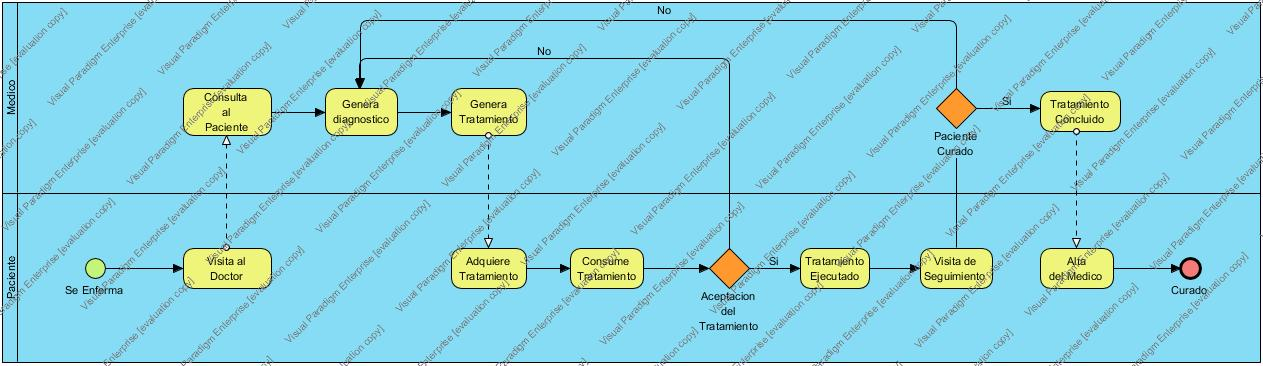
\includegraphics[width=1.1\textwidth]{images/cap2/ProcesoMedico}
	\caption{Proceso médico en la actualidad} \label{fig:proceso1}
\end{figure}

En cambio con el uso de la aplicación como se muestra en la imagen \ref{fig:proceso2} podemos notar como el uso de las nuevas tecnologías ayuda tanto a los pacientes como a los médicos.

\begin{figure}[htb]
	\centering
	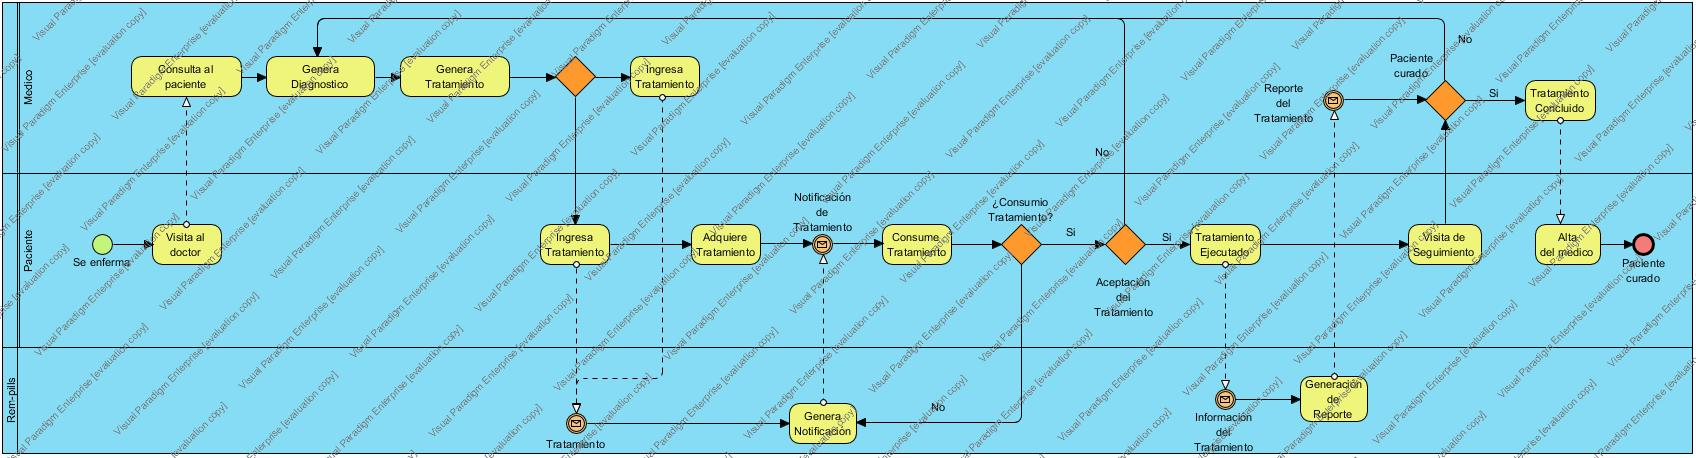
\includegraphics[width=1.1\textwidth]{images/cap2/RemPillstratamiento}
	\caption{Proceso médico con ayuda de la aplicación} \label{fig:proceso2}
\end{figure}


\section{Casos de uso}
En el análisis realizado para la aplicación Rem-Pills se identificaron los siguientes casos de uso como se muestra en la figura\ref{fig:casosdeuso}
\begin{figure}[htb]
	\centering
	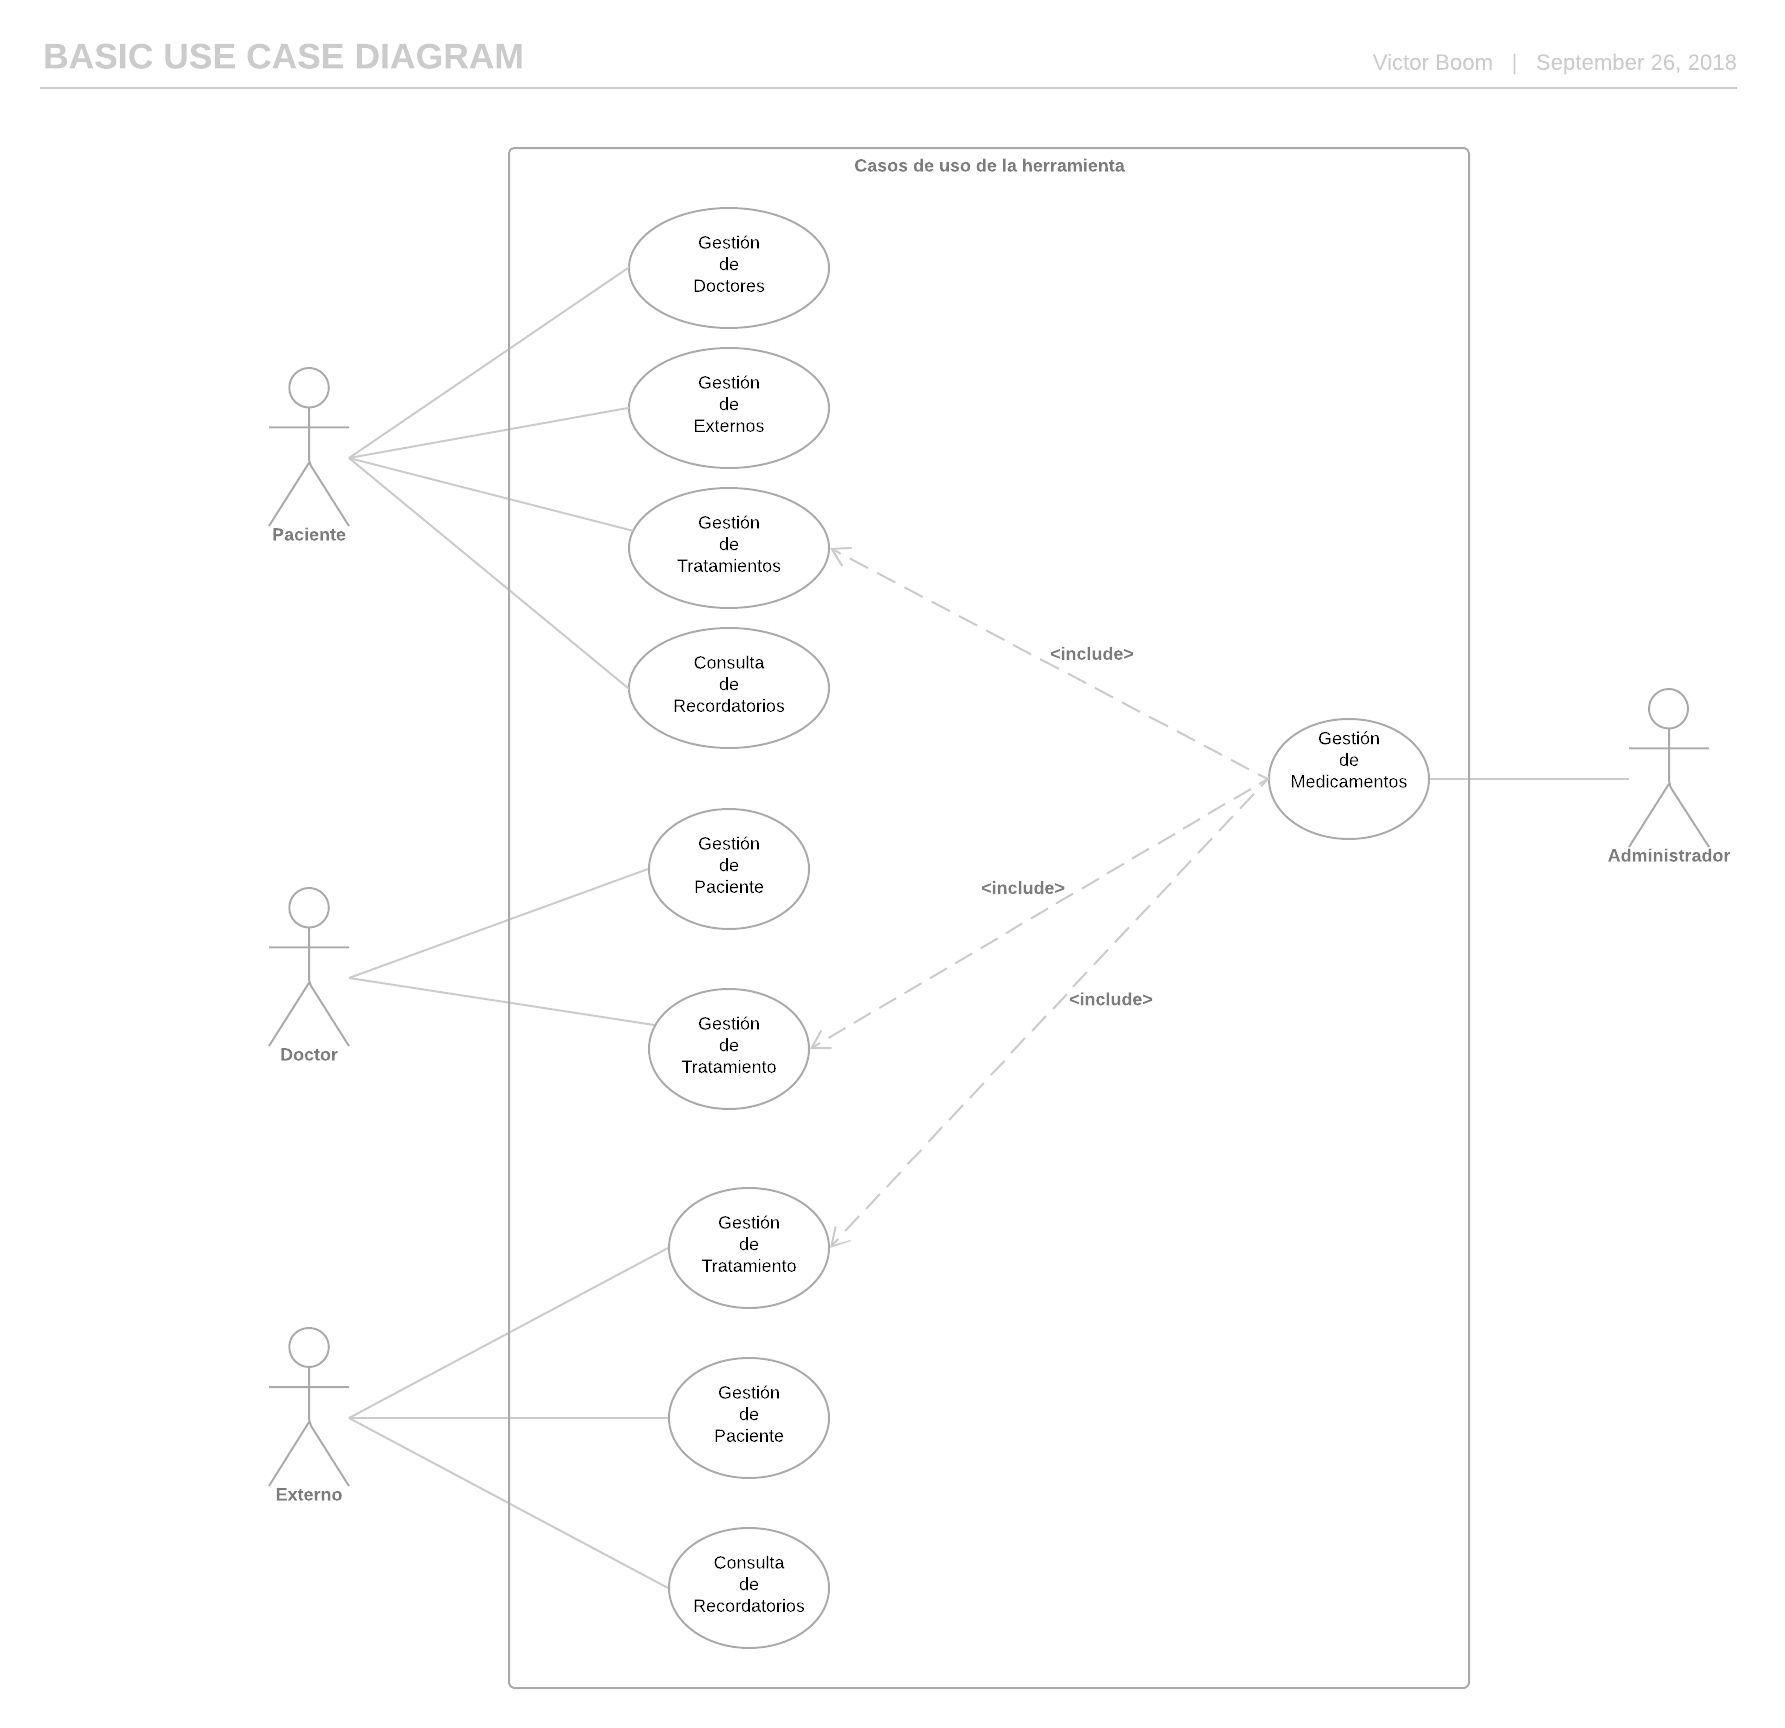
\includegraphics[width=1.1\textwidth]{images/cap2/casosdeuso}
	\caption{Proceso médico con ayuda de la aplicación} \label{fig:casosdeuso}
\end{figure} 
La aplicación cuenta con los siguientes casos de uso, que se explicaran a detalle a continuación :
\begin{itemize}
	
	\item Gestión de Doctores:
		\begin{itemize}
			\item Agregar Doctor: Este caso de uso permitirá a un paciente agregar a un doctor.
			\item Eliminar Doctor: Este caso de uso permitirá a un paciente a eliminar a un doctor.
			\item Consultar Doctor: Este caso de uso permitirá a un paciente a consultar información relevante de su doctor.
		\end{itemize}
	Como se puede notar el caso de uso \textbf{Gestión de Doctores} engloba tres tipos de casos de uso distintos.
	
	\item Gestión de Auxiliares:
	\begin{itemize}
		\item Agregar Auxiliar: Este caso de uso permitirá a un paciente agregar a un auxiliar.
		\item Eliminar Auxiliar: Este caso de uso permitirá a un paciente a eliminar a un auxiliar.
		\item Consultar Axiliar: Este caso de uso permitirá a un paciente a consultar información relevante de su auxiliar.
	\end{itemize}
	Como se puede notar el caso de uso \textbf{Gestión de Auxiliar} engloba tres tipos de casos de uso distintos.
	
	\item Gestión de Pacientes:
	\begin{itemize}
		\item Agregar Paciente: Este caso de uso permitirá a un doctor y a un auxiliar agregar a un doctor.
		\item Eliminar Paciente: Este caso de uso permitirá a un doctor y a un auxiliar a eliminar a un doctor.
		\item Consultar Paciente: Este caso de uso permitirá a un un doctor y a un auxiliar a consultar información relevante de su doctor.
	\end{itemize}
	Como se puede notar el caso de uso \textbf{Gestión de Pacientes} engloba tres tipos de casos de uso distintos.
	
	\item Gestión de Tratamientos: 
	\begin{itemize}
		\item Agregar Tratamiento: Este caso de uso permite tanto al paciente, doctor y auxiliar agregar un tratamiento.
		\item Eliminar Tratamiento: Este caso de uso permite tanto al paciente, doctor, y auxiliar eliminar un tratamiento existente.
		\item Consultar Tratamiento: Este caso de uso permite tanto al paciente, doctor y auxiliar consultar un tratamiento existente.
		\item Editar Tratamiento: Este caso de uso permite tanto al paciente, doctor, y auxiliar editar un tratamiento existente.
	\end{itemize}
	
	\item Gestión de Recordatorios:
	\begin{itemize}
		\item Editar recordatorio
		\item Consultar recordatorio
	\end{itemize}
	
	\item Gestión de Medicamentos:
	\begin{itemize}
		\item Agregar medicamento:
		\item Eliminar medicamento:
		\item Editar medicamento:
		\item Consultar medicamento:
	\end{itemize}
\end{itemize}